%!TEX root = thesis.tex
\chapter{Analysis} % (fold)
\label{ch:analysis}
This section analyses the user preferences and identifies with features should be modelled as personalisation constraints. I also seeks to define the default setting that consists the general model for a good digital newspaper.

The focus of automatically generating the editorial mix introduces circumstances about the similarities between articles. These will consist the content constraints of the system along with those determined by user preferences. Therefore the constraints that belongs to composition conditions must be presented/defined.

prerequisites:
\begin{itemize}
	\item 14.732x20.828cm \cite[p. 1]{FULLTEXT01.pdf}
	\item A5 (A4 if reducible) \cite[p. 6-7]{kristin_fredrik.pdf}
	\item reader knows about constraints
	\item relevance feedback introduced (click on article, time spend reading it and scroll)
	\item argument that transparency of the general model is enough for the user to provide settings \cite[p. 7]{gervasum2001ws.pdf}
\end{itemize}

\section{User Needs}
This section will define the user needs for the application.

\subsection{Business Case}

\subsubsection{Need}
User value: personal quality and up-to-date stories enriched with quality images. This means that content providers should be chosen/verified. Same navigation as actual newspapers, but faster and with endless more content. Instantly up-to-date. Adaptive layout. Adjustable user profile.

\subsubsection{Approach}
personalised content + composition.

Constraint Programming: fast computation - good for optimal solutions, describes the generic solution in stead of how to solve or find it, very easy to tailor the problem definition of the solution and adjust it and even let users make the adjustments - transparency.

Content providers can get to know their readers preferences better and improve the provided content.

\subsubsection{Benefit Per Cost}
Revenue flow: Content providers are paid. Income from advertisers (scattered \cite[p. 6-7]{kristin_fredrik.pdf}) and users. Income from selling user behaviour patterns and targeted commercials.

\subsubsection{Competition}
Flip board, Wired magazine, zite and app with actual editors affiliated.

\todonote{Which design choices to focus on?}

\begin{itemize}
	\item ``open, turn pages, chose article, read and return'' \cite[p. 6]{FULLTEXT01.pdf}
	\item both general and personal news (collaborate filtering solves that some news are not received, but are universally interesting \cite{fulltext.pdf})
	\item full screen display of article
	\item images + video? adjustable
	\item graphical/textual content ratio
	\item opens in front page view (summery of newspaper 8 articles) \cite[p. 8]{kristin_fredrik.pdf}
	\item put in personalised sections
	\item back page, funnies?
	\item section headline \cite[p. 6-7]{kristin_fredrik.pdf}
	\item article headlines
	\item article summaries / extracts \cite{fulltext.pdf}
	\item menu w. section headlines \cite[p. 8]{kristin_fredrik.pdf}
	\item page numbers \cite[p. 6-7]{kristin_fredrik.pdf}
	\item page turn
	\item press ``like'' or key word based user profile (mark self or highlighted? right click to add): positive + negative list (keywords+categories \cite{10-1-1-19-5583}, \cite{fulltext.pdf} and \cite{gervasum2001ws.pdf})
	\item adjust variables
	\item share social network
	\item share directly (grey out the ones who have read it)
	\item comment
	\item see friends comments
\end{itemize}

\subsection{Technical Requirements}
\begin{itemize}
	\item ``the clear overview of content, including a beginning and an end, the ease of use, typography and design'' \cite[p. 7]{FULLTEXT01.pdf}
	\item familiarity in design from printed paper \cite[p. 7]{FULLTEXT01.pdf}
	\item  ``news valuation, e.g. positioning of lead story'' \cite[p. 7]{FULLTEXT01.pdf}
	\item  mobility \cite[p. 7]{FULLTEXT01.pdf}
	\item  continuous updates \cite[p. 7]{FULLTEXT01.pdf}
	\item  ability to search \cite[p. 7]{FULLTEXT01.pdf}
	\item  ``easy and intuitive navigation'' \cite[p. 7]{FULLTEXT01.pdf}
	\item add video and sound \cite[p. 7]{FULLTEXT01.pdf}
	\item Landscape + portrait \cite[p. 6-7]{kristin_fredrik.pdf}
	\item touch screen interaction \cite[p. 6-7]{kristin_fredrik.pdf}
	\item Design+layout from printed newspaper \cite{hcii2005_1004.pdf}
	\item Functionality from online newspaper \cite{hcii2005_1004.pdf}
	\item Name of columnist \cite[p. 4]{gervasum2001ws.pdf}
	\item Transparency of implicit relevance feedback (see/modify current weights of categories) \cite[p. 7]{gervasum2001ws.pdf}
	\item dynamic short-term + static long-term user profile \cite{10-1-1-19-5583}, \cite{fulltext.pdf} and \cite{gervasum2001ws.pdf}
	\item relevance feedback \cite{10-1-1-19-5583}, \cite{fulltext.pdf} and \cite{gervasum2001ws.pdf}
\end{itemize}

In which period of time is an article relevant to a user? Maybe if it is still available, then it is still interesting - new approaches or discussion about the subject might arise. How do we control that a news item is not missed? Keep index of what has been viewed in addition to what has been read.

%/Library/Frameworks/Python.framework/Versions/3.2/bin:/Library/Frameworks/Python.framework/Versions/2.6/bin:/Library/Frameworks/Python.framework/Versions/2.7/bin:/usr/local/bin:/Users/ml/.local/bin:/usr/texbin/:/usr/bin:/bin:/usr/sbin:/sbin:/usr/local/bin:/usr/local/git/bin:/usr/texbin:/usr/X11/bin:/opt/local/bin:/opt/local/sbin

%/usr/bin:/bin:/usr/sbin:/sbin:/usr/local/bin:/usr/local/git/bin:/usr/texbin:/usr/X11/bin:/opt/local/bin:/opt/local/sbin

%/Library/Frameworks/Python.framework/Versions/3.2/bin:/Library/Frameworks/Python.framework/Versions/2.6/bin:/Library/Frameworks/Python.framework/Versions/2.7/bin:/usr/local/bin:/Users/ml/.local/bin:/usr/texbin/:/usr/bin:/bin:/usr/sbin:/sbin:/usr/local/bin:/usr/local/git/bin:/usr/texbin:/usr/X11/bin:/opt/local/bin:/opt/local/sbin
%aggregator
%reader
%constraint
%news
%social
%now
%fluid layout
%flow
%papr
%editor

\section{Interface}
\subsection{Typeface}
``How users read the web: They don't. They scan the page, picking out individual words and sentences'', %\cite{Jakob Nielsen}
\todonote{Jakob Nielsen cite}

Colour scheme: \url{http://colorschemedesigner.com/#0042b1Tw0w0w0}

\begin{figure}[h!tp]
	\centering
		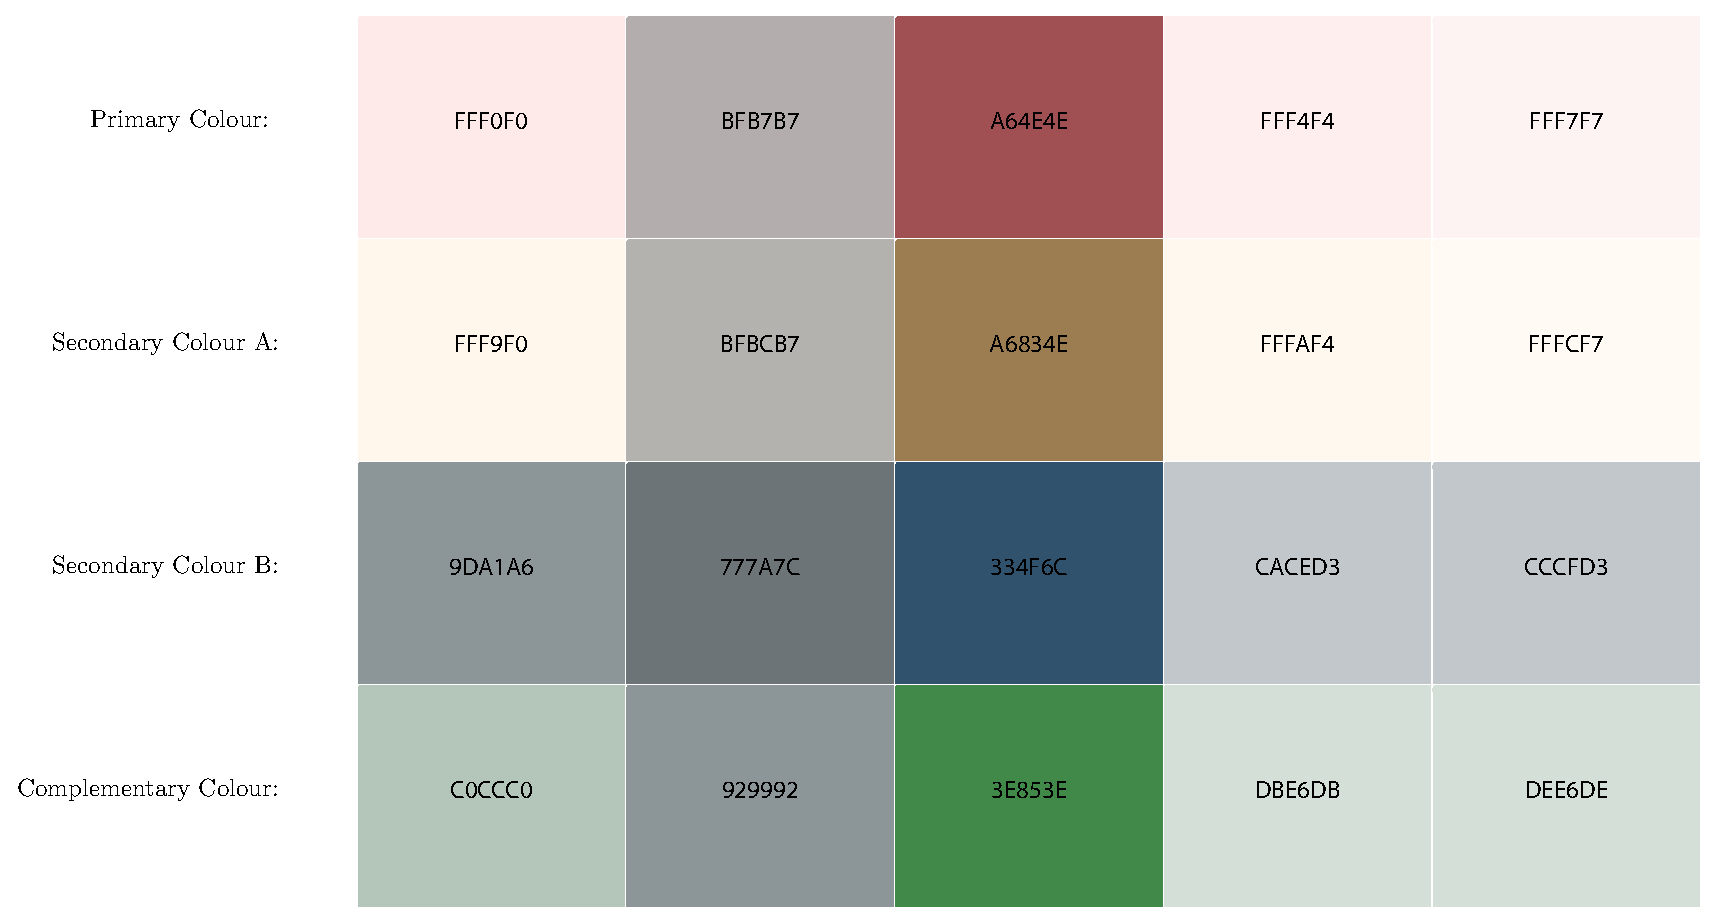
\includegraphics[width=.45\textwidth]{img/colour-scheme.eps}
	\caption{Colour scheme of the interface \protect\cite{colorschemedesigner.com}}
	\label{fig:colour-scheme}
\end{figure}
\todonote{colorschemedesigner.com cite}

\section{Test}




\section{Constraints}
The constraints can be divided into groups: layout-/content-based, global/topic/neighbouring, 


Technical argumentation for choices.
Business case argumentation for choices (user needs).
Reference to written articles about design choices - navigation: sections + headlines, 

\subsection{Layout Constraints}
first focus: layout + one sections

3? columns
images/no image
base layout



\subsection{Content Constraints}
Content similarity relationships:
article vs. neighbouring articles
article vs. containing section/topic
article vs. whole newspaper

``[...] it was found that the best eight-item  mix within an issue was not necessarily composed of the eight highest-readership items in that issue.'' \cite{EditorsDilemma} (maximum audience coverage, which is no longer an issue due to personalisation)

\begin{align*}
\mathcal{C} &=	\begin{Bmatrix}
					\texttt{all\_different}(a_i),\\
					\texttt{sim}(a_i, a_{i+1}, 0.7, 0.9), \\
					\texttt{sim}(a_i, a_{i-1}, 0.7, 0.9), \\
					\texttt{sim}(a_i, a_j, 0.3, 0.9)
					%artists_i \ne artists_{i-1} \wedge artists_i \ne artists_{i+1},\\
					%album_i \ne album_{i-1} \wedge album_i \ne album_{i+1},\\
					%\texttt{all\_different}(place_i),\\
					tempo_i < tempo_{i+1} + 10 \wedge tempo_i < tempo_{i-1} + 10 \wedge\\
					tempo_i > tempo_{i-1} - 10 \wedge tempo_i > tempo_{i+1} - 10,\\
					%tempo_i < + 5 \cdot length \cdot tempo_j \wedge\\
					%tempo_i > - 5 \cdot length \cdot tempo_j\ \textbf{for}\ i \ne j,\\
					%keys_i = keys_i \vee keys_i = keys_i \pm 1 \vee keys_i = keys_i \pm 12
				\end{Bmatrix}
\end{align*}


\todonote{AIRussel p. 207 preference constraints. can often be encoded as costs on individual variable assignments. Solved either path-based or local.
p. 216 Minimum-remaining-values, p. 217 Least-constraining-value.}

\section{Test Results}
long layout

Stumbleupon - Collaborate filtering for recommendation

% section analysis (end)
